\documentclass[aspectratio=169]{beamer}
%[handout]

\usetheme[progressbar=frametitle]{metropolis}
\usepackage{appendixnumberbeamer}

\usepackage[utf8]{inputenc}
\usepackage[T1]{fontenc}

\usepackage[brazil]{babel}
\usepackage[outputdir=..]{minted}
\usepackage{xcolor}
\usepackage{soul} % strikethrough
\usepackage{advdate}
\usepackage{graphicx}
\graphicspath{{figs/}}
\usepackage{graphbox}

\usepackage[ampersand]{easylist}

\usepackage{multirow}
\usepackage{multicol}
\usepackage{subcaption}

\usepackage{pgf,tikz}
\usetikzlibrary{shapes,arrows,positioning}
\usetikzlibrary{circuits.logic.US}
\usetikzlibrary{matrix,calc}

\usepackage{karnaugh-map}

\usepackage{pgfpages}
\setbeameroption{hide notes} % Only slides
% \setbeameroption{show only notes} % Only notes
% \setbeameroption{show notes on second screen=right} % Both

% \graphicspath{{../figs/}}

\definecolor{bgc}{rgb}{0.95,0.9,0.95}
\definecolor{links}{HTML}{2A7F7F}
\hypersetup{colorlinks,linkcolor=,urlcolor=links}

\newminted{verilog}{fontsize=\scriptsize, 
    linenos,
    numbersep=8pt,
    bgcolor=bgc,
    tabsize=4,
    framesep=3mm} 
    %frame=lines,

\newcommand{\verilog}[1]{\verilogf{#1}{\footnotesize}}

\newcommand{\verilogf}[2]{\inputminted[fontsize=#2, 
    linenos,
    tabsize=2,
    numbersep=4pt,
    bgcolor=bgc,
    framesep=3mm]{verilog}{../codes/#1.v}
}

\newminted{nasm}{fontsize=\scriptsize, 
		   linenos,
		   numbersep=8pt,
           bgcolor=bgc,
		   framesep=3mm} 

\usepackage{booktabs}
\usepackage[scale=2]{ccicons}

\usepackage{pgfplots}
\usepgfplotslibrary{dateplot}

\usepackage{hyperref}


\usepackage{xspace}
\newcommand{\themename}{\textbf{\textsc{metropolis}}\xspace}



\usepackage{pifont}% http://ctan.org/pkg/pifont
\newcommand{\cmark}{\ding{51}}%
\newcommand{\xmark}{\ding{55}}%

% \tiny	
% \scriptsize
% \footnotesize
% \small	
% \normalsize	
% \large	
% \Large	
% \LARGE	
% \huge	
% \Huge	



\newminted{python}{fontsize=\scriptsize, 
		   linenos,
		   breaklines,
		   numbersep=8pt,
           tabsize=2,
		   framesep=3mm} 
		   
\newminted{verilog}{fontsize=\scriptsize, 
		   linenos,
		   breaklines,
		   numbersep=8pt,
           tabsize=2,
		   framesep=3mm} 
		   




\definecolor{bgc}{rgb}{0.95,0.9,0.95}
\definecolor{links}{HTML}{2A7F7F}
\hypersetup{colorlinks,linkcolor=,urlcolor=links}


% \usepackage[style=apa]{biblatex}
% \addbibresource{mm.bib}


% \author{\large Prof. Ricardo Menotti (\href{mailto:menotti@ufscar.br}{menotti@ufscar.br})}

\newcommand{\newauthor}[2]{
  \parbox{0.50\textwidth}{
    \texorpdfstring
      {
        \centering
        \small #1 \newline
        {\scriptsize{\urlstyle{same}\href{mailto:#2}{#2}\urlstyle{tt}}}
      }
      {#1} \newline
  }
}

\author{
  \newauthor{Prof. Ricardo Menotti}{menotti@ufscar.br}
\and \newauthor{Prof. Luciano de Oliveira Neris}{lneris@ufscar.br}  
%\and \newauthor{Prof. Artino Quintino da Silva Filho}{artino@ufscar.br}
% \and \newauthor{Prof. Maurício Figueiredo}{mauricio@ufscar.br}
% \and \newauthor{Prof. Edilson Kato}{kato@ufscar.br}
% \and \newauthor{Prof. Roberto Inoue}{rsinoue@ufscar.br}
}

\date{Atualizado em: \today}

\institute{\large \textbf{Departamento de Computação} \\
Centro de Ciências Exatas e de Tecnologia \\
Universidade Federal de São Carlos}

\title{Lógica Digital (1001351)}

\titlegraphic{\hfill
\includegraphics[height=1.5cm]{LogoUfscar}}



\subtitle{Circuitos Sequenciais: Registradores} % 

\begin{document}

\begin{frame}
	\titlepage
\end{frame} 

\section{Circuitos Sequenciais}

\begin{frame}{Objetivos}   %\centering
    Nesta aula vamos aprender sobre:
    \begin{itemize}
        \item Registradores, os quais armazenam vários bits;
        \item Registradores de deslocamento;
        \item Contadores de vários tipos.
    \end{itemize}
\end{frame}

\begin{frame}{Registrador de deslocamento}   \centering
    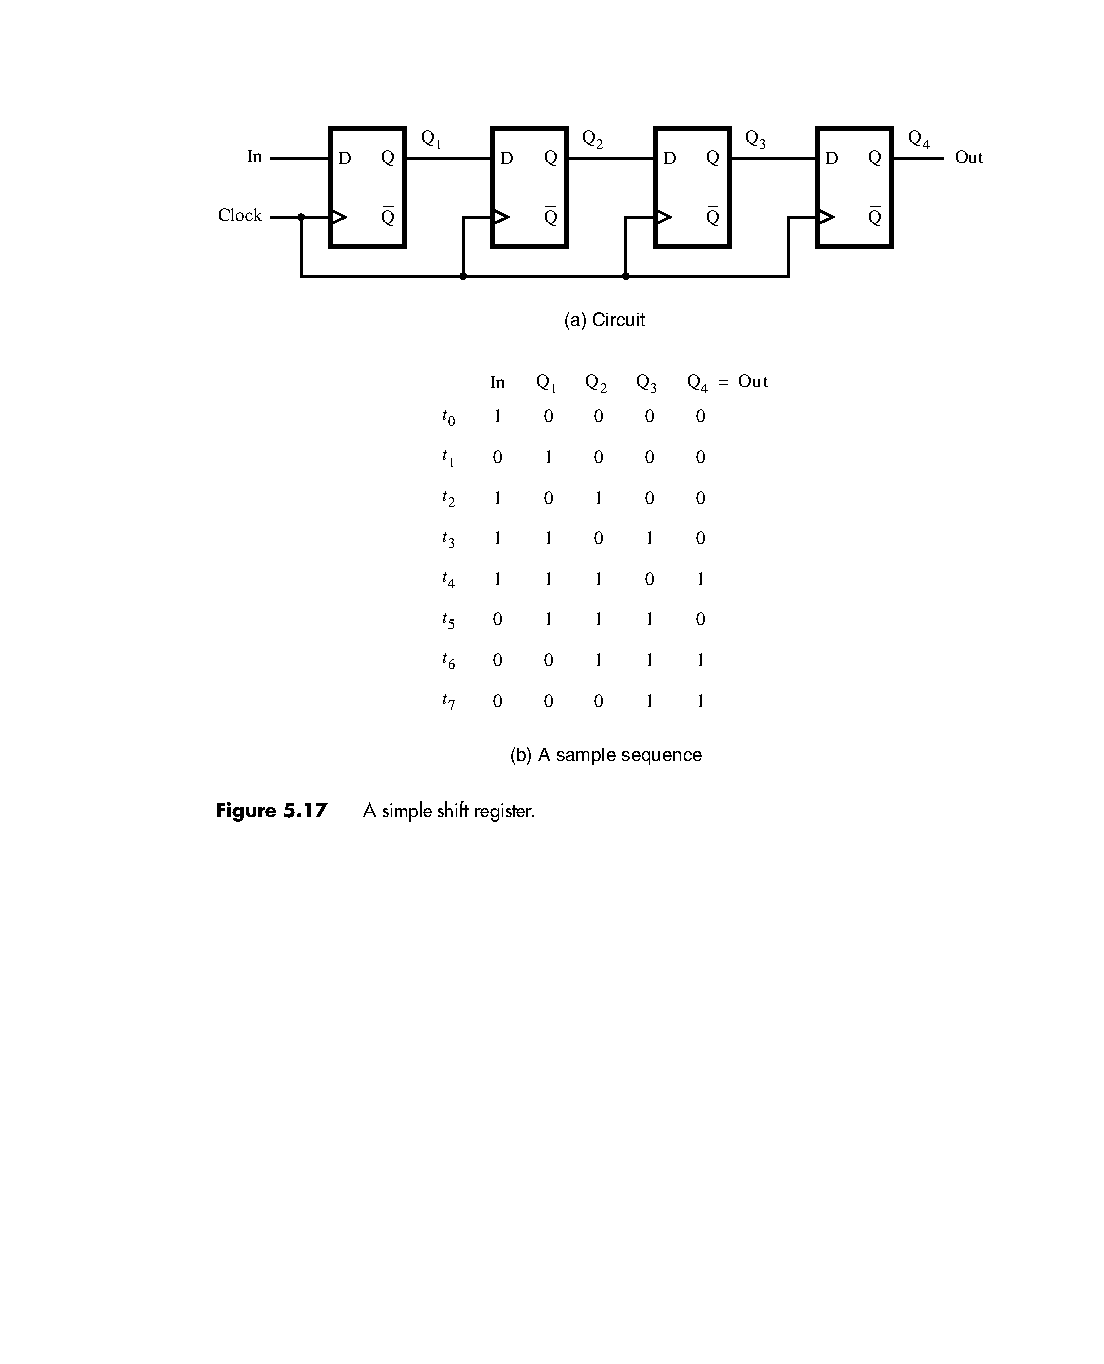
\includegraphics[height=.95\textheight]{VerilogFig5_17} \\
\end{frame}

\begin{frame}{Registrador de deslocamento com carga paralela}   \centering
    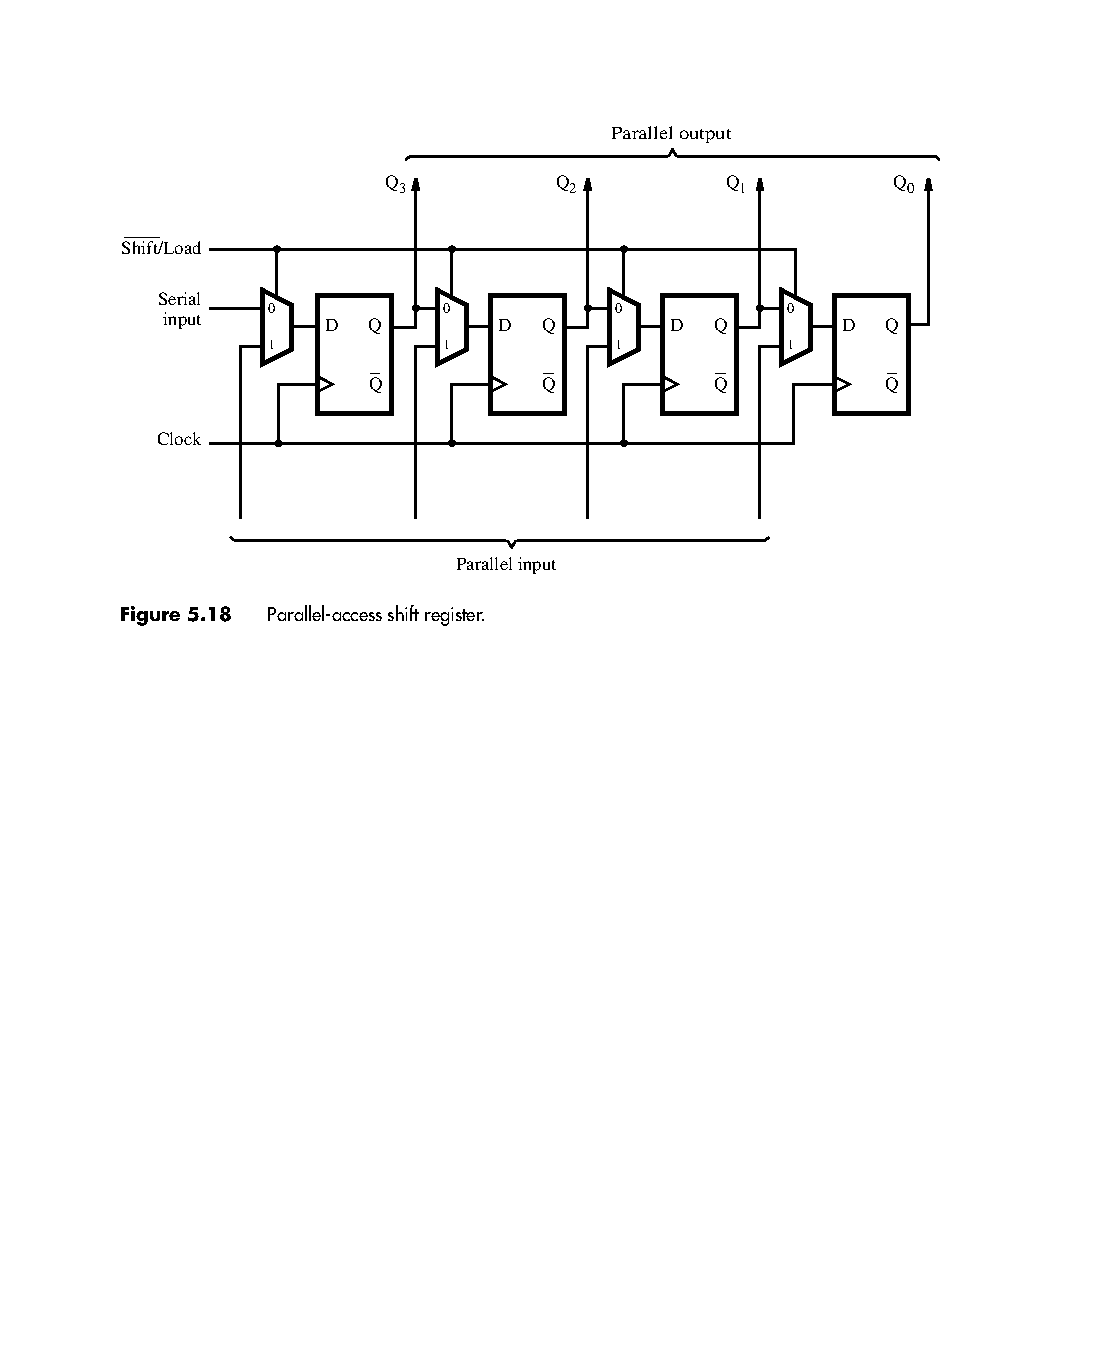
\includegraphics[height=.95\textheight]{VerilogFig5_18} \\
\end{frame}

\begin{frame}{Contador de três bits}   \centering
    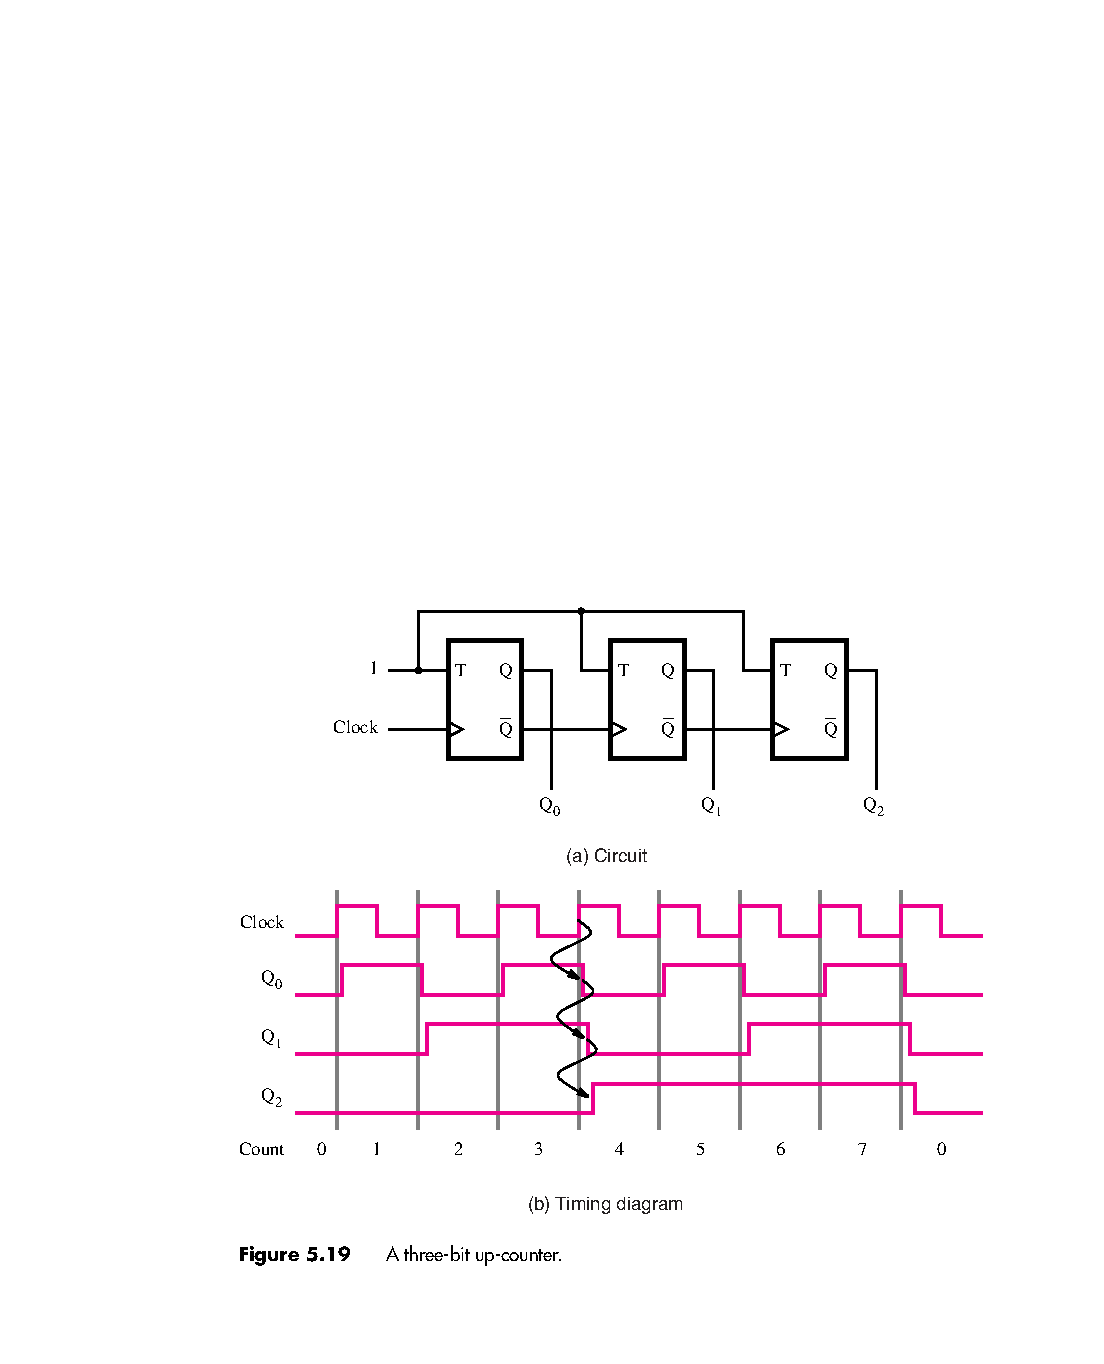
\includegraphics[height=.95\textheight]{VerilogFig5_19} \\
\end{frame}

\begin{frame}{Contador de três bits (decremento)}   \centering
    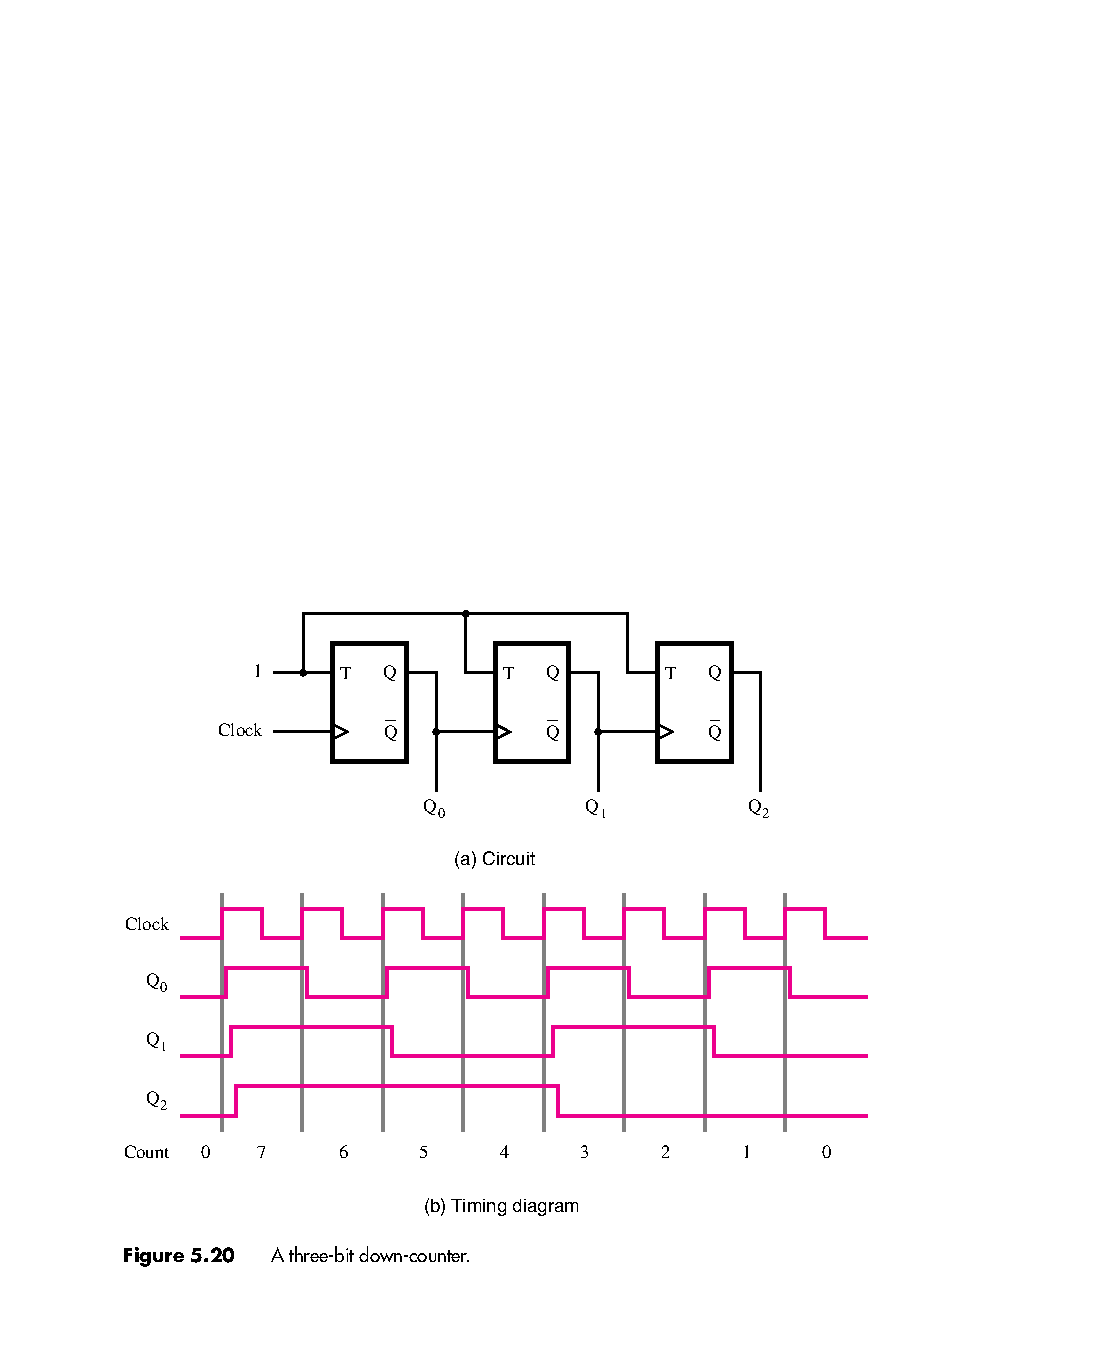
\includegraphics[height=.95\textheight]{VerilogFig5_20} \\
\end{frame}

\begin{frame}{}   \centering
	\begin{columns}
        \column{0.6\textwidth}
    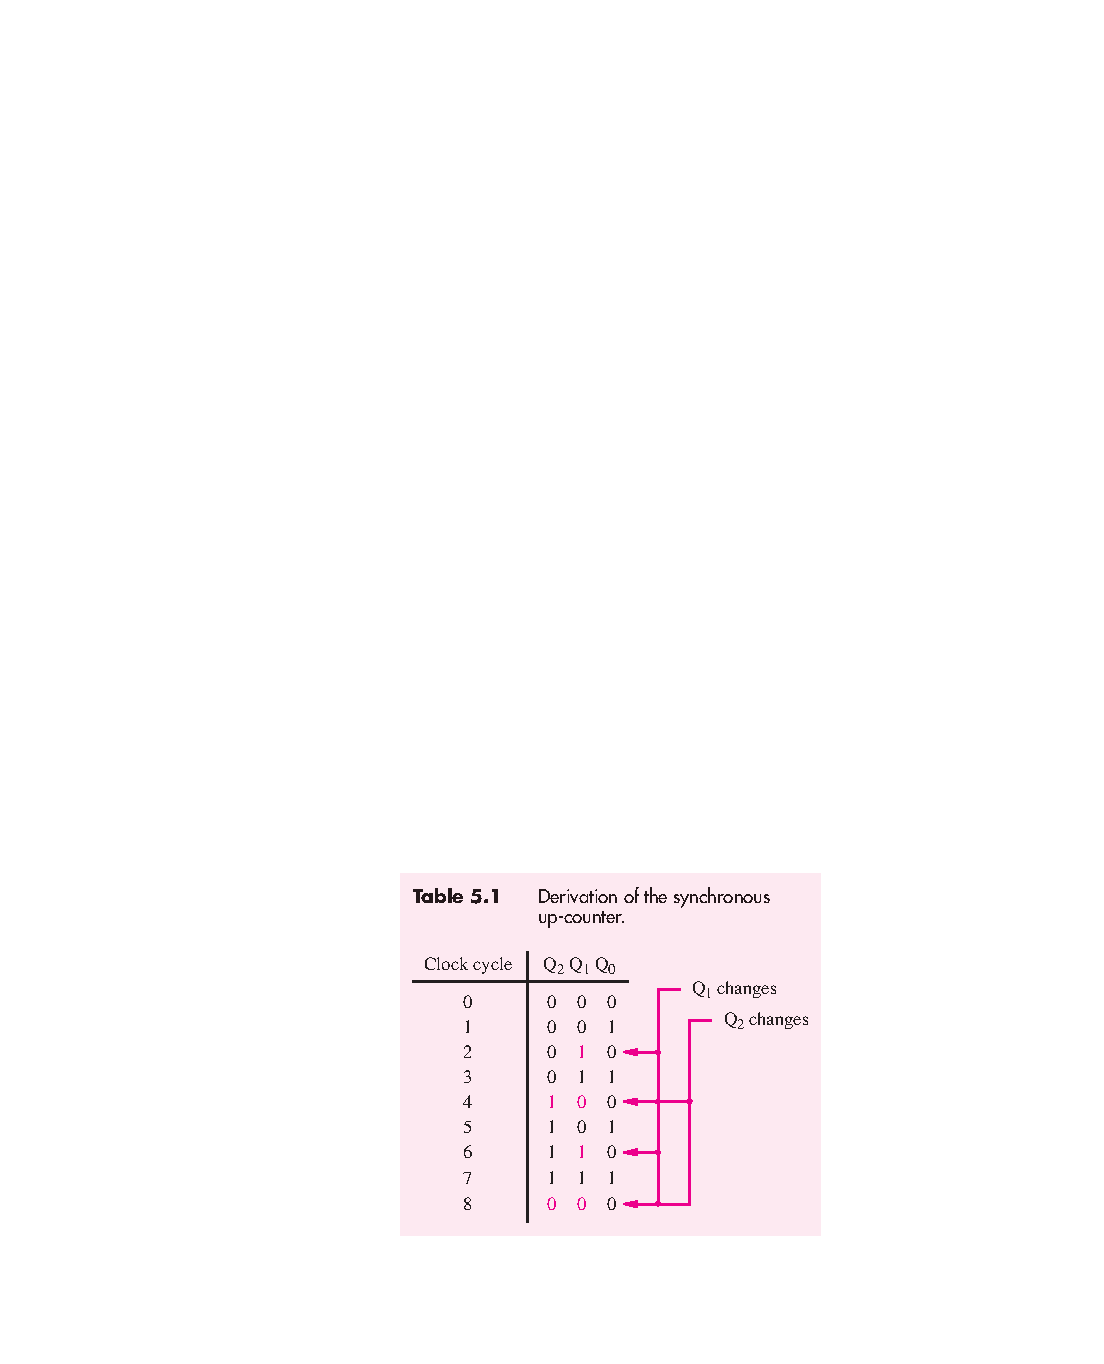
\includegraphics[width=\textwidth]{VerilogTab5_1} \\
        \column{0.4\textwidth}
        $T_0 = 1$ \\
        $T_1 = Q_0$ \\
        $T_2 = Q_0Q_1$ \\
        $T_3 = Q_0Q_1Q_2$ \\
        . \\
        . \\
        . \\
        $T_n = Q_0Q_1...Q_{n-1}$ \\
    \end{columns}
\end{frame}

\begin{frame}{Contador de 4 bits síncrono}   \centering
    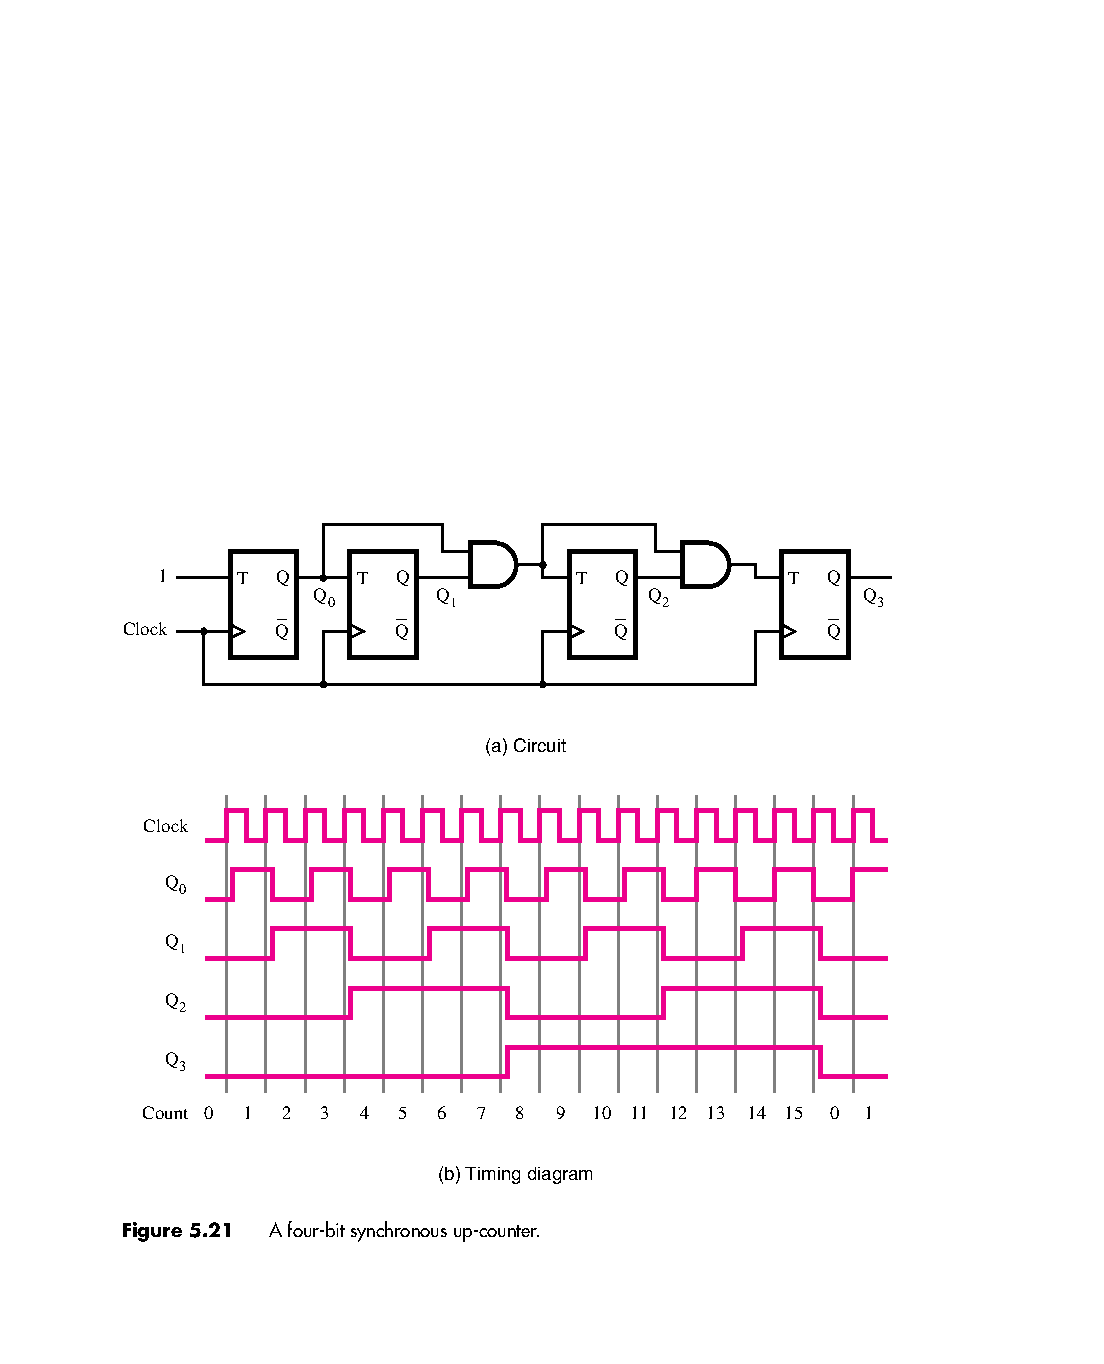
\includegraphics[height=.95\textheight]{VerilogFig5_21} \\
\end{frame}

\begin{frame}{Contador de 4 bits síncrono com \textit{enable}}   \centering
    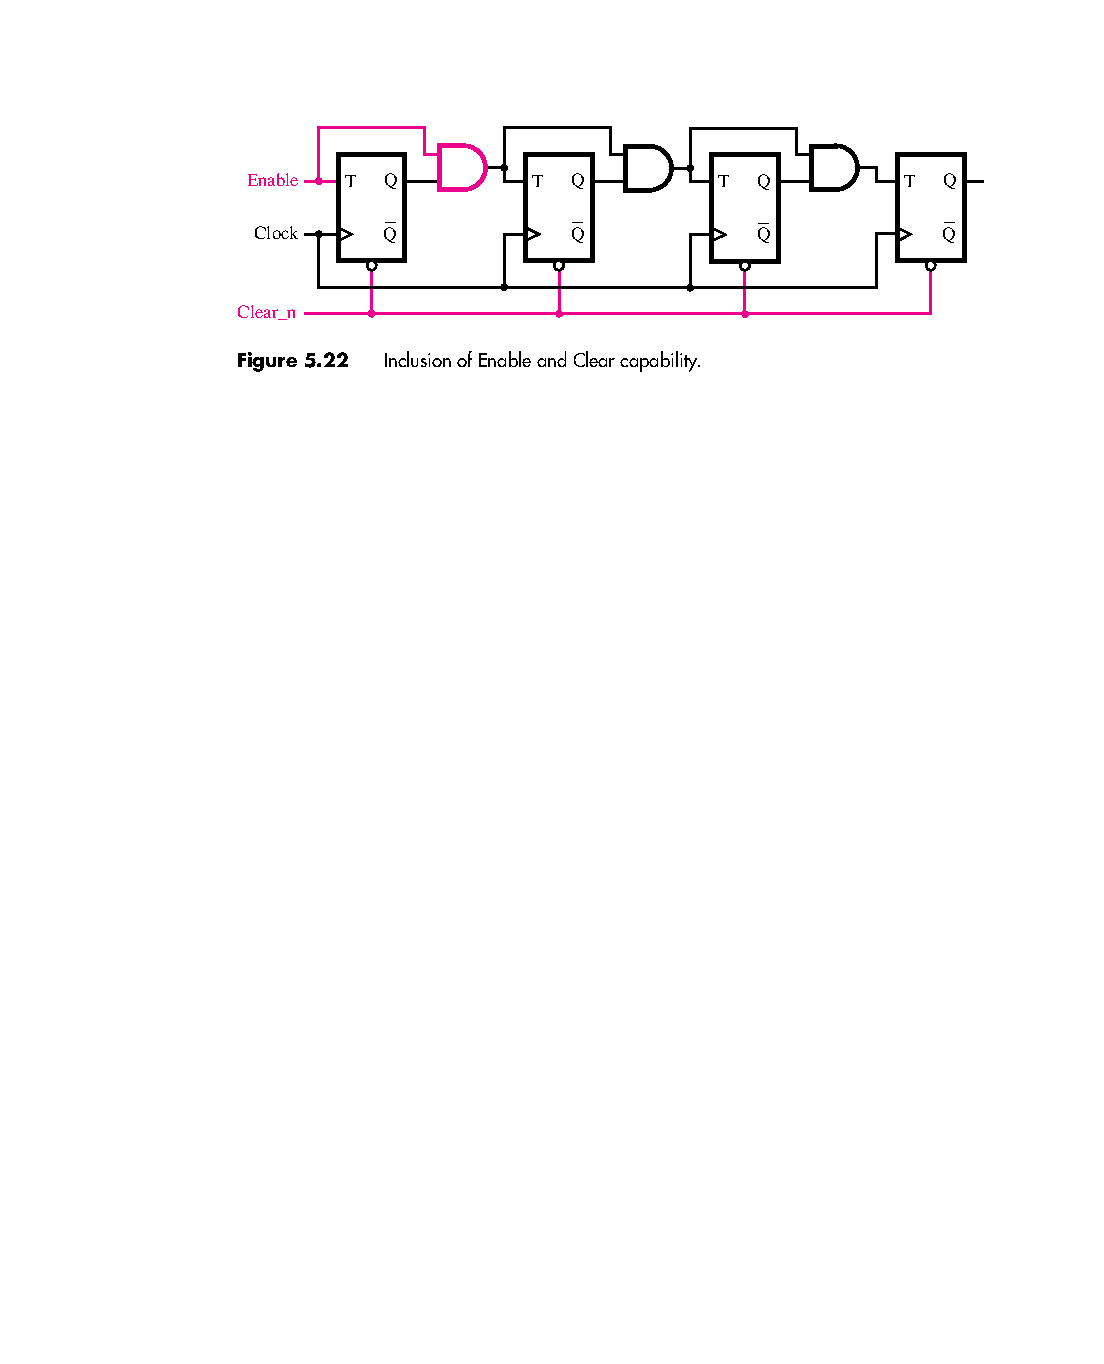
\includegraphics[width=\textwidth]{VerilogFig5_22} \\
\end{frame}

\begin{frame}{Usando flip-flops do tipo D}   \centering
	\begin{columns}
        \column{0.6\textwidth}
    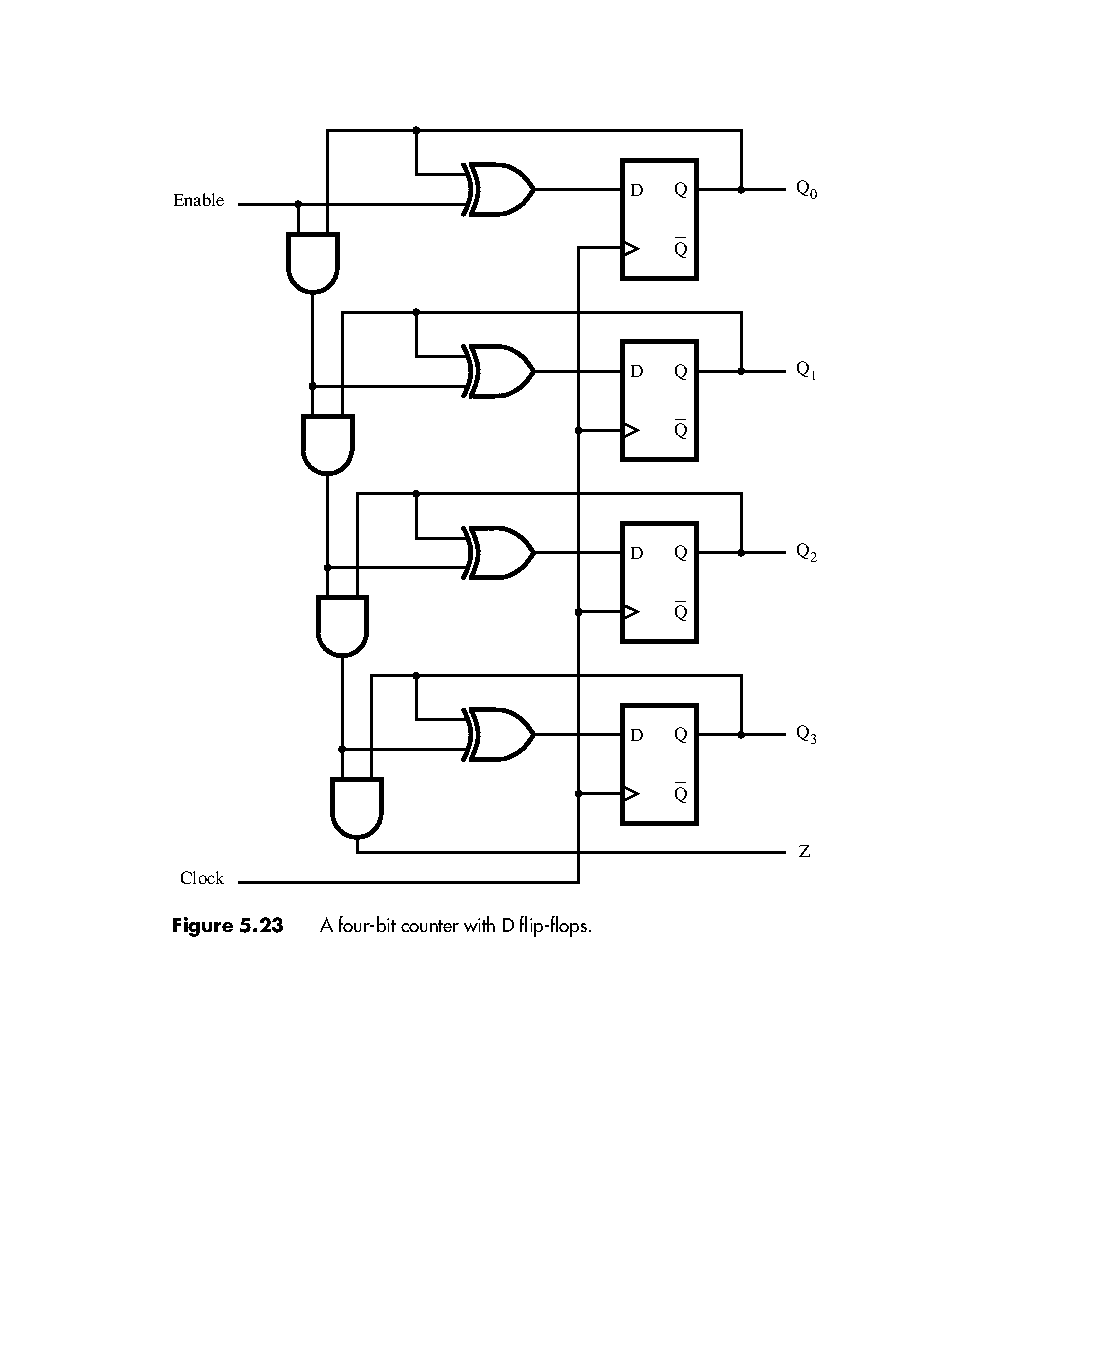
\includegraphics[height=.95\textheight]{VerilogFig5_23} \\
        \column{0.4\textwidth}
        $D_0 = Q_0 \oplus 1 = \overline{Q}_0$ \\
        $D_1 = Q_1 \oplus Q_0$ \\
        $D_2 = Q_2 \oplus Q_1Q_0$ \\
        $D_3 = Q_3 \oplus Q_2Q_1Q_0$ \\
        . \\
        . \\
        . \\
        $D_i = Q_i \oplus Q_{i-1}Q_{i-2}...Q_1Q_0$ \\
    \end{columns}
\end{frame}

\begin{frame}{Contador com carga paralela}   \centering
    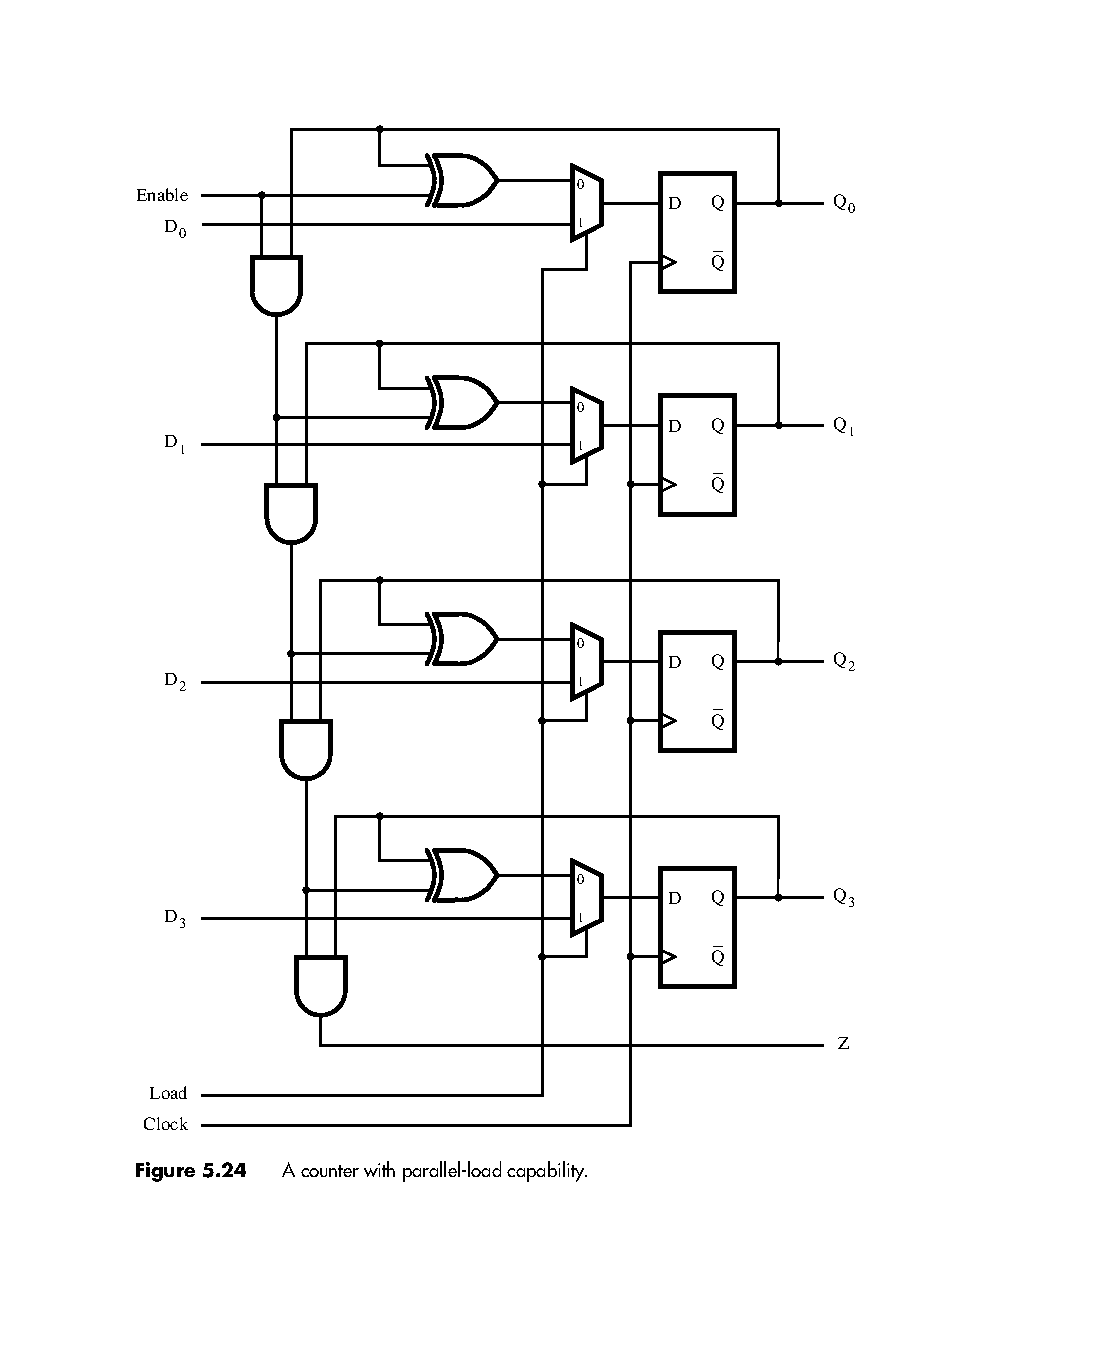
\includegraphics[height=.95\textheight]{VerilogFig5_24} \\
\end{frame}

\begin{frame}{Contador módulo-6 com reset síncrono}   \centering
    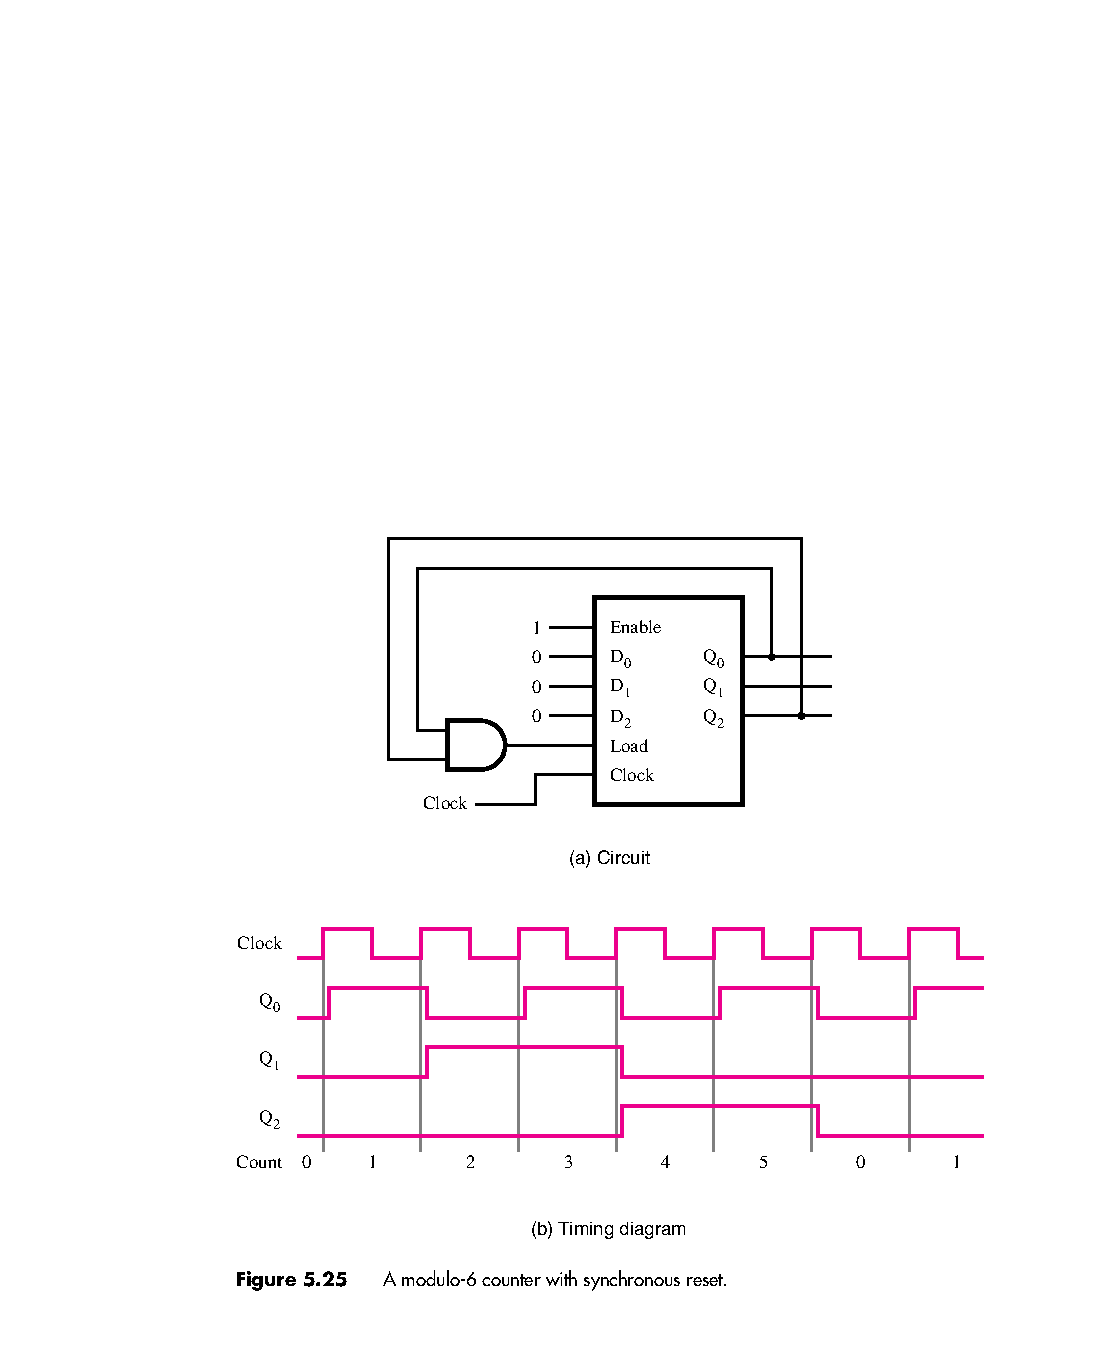
\includegraphics[height=.95\textheight]{VerilogFig5_25} \\
\end{frame}

\begin{frame}{Contador módulo-6 com reset assíncrono}   \centering
    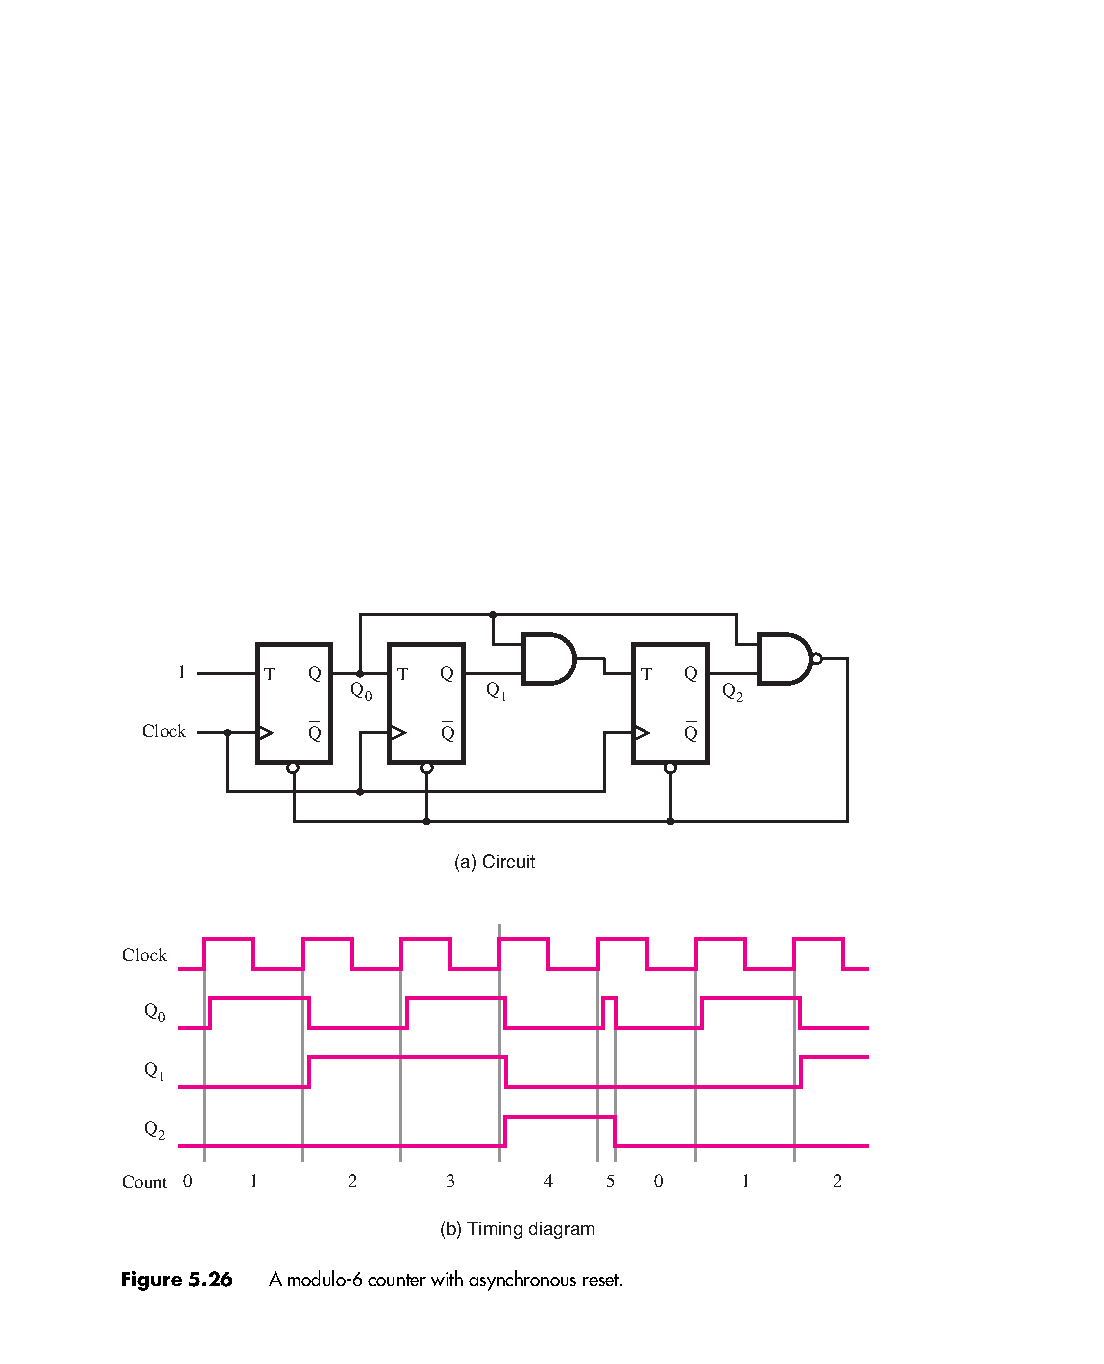
\includegraphics[height=.95\textheight]{VerilogFig5_26} \\
\end{frame}

\begin{frame}{Contador BCD de dois dígitos}   \centering
    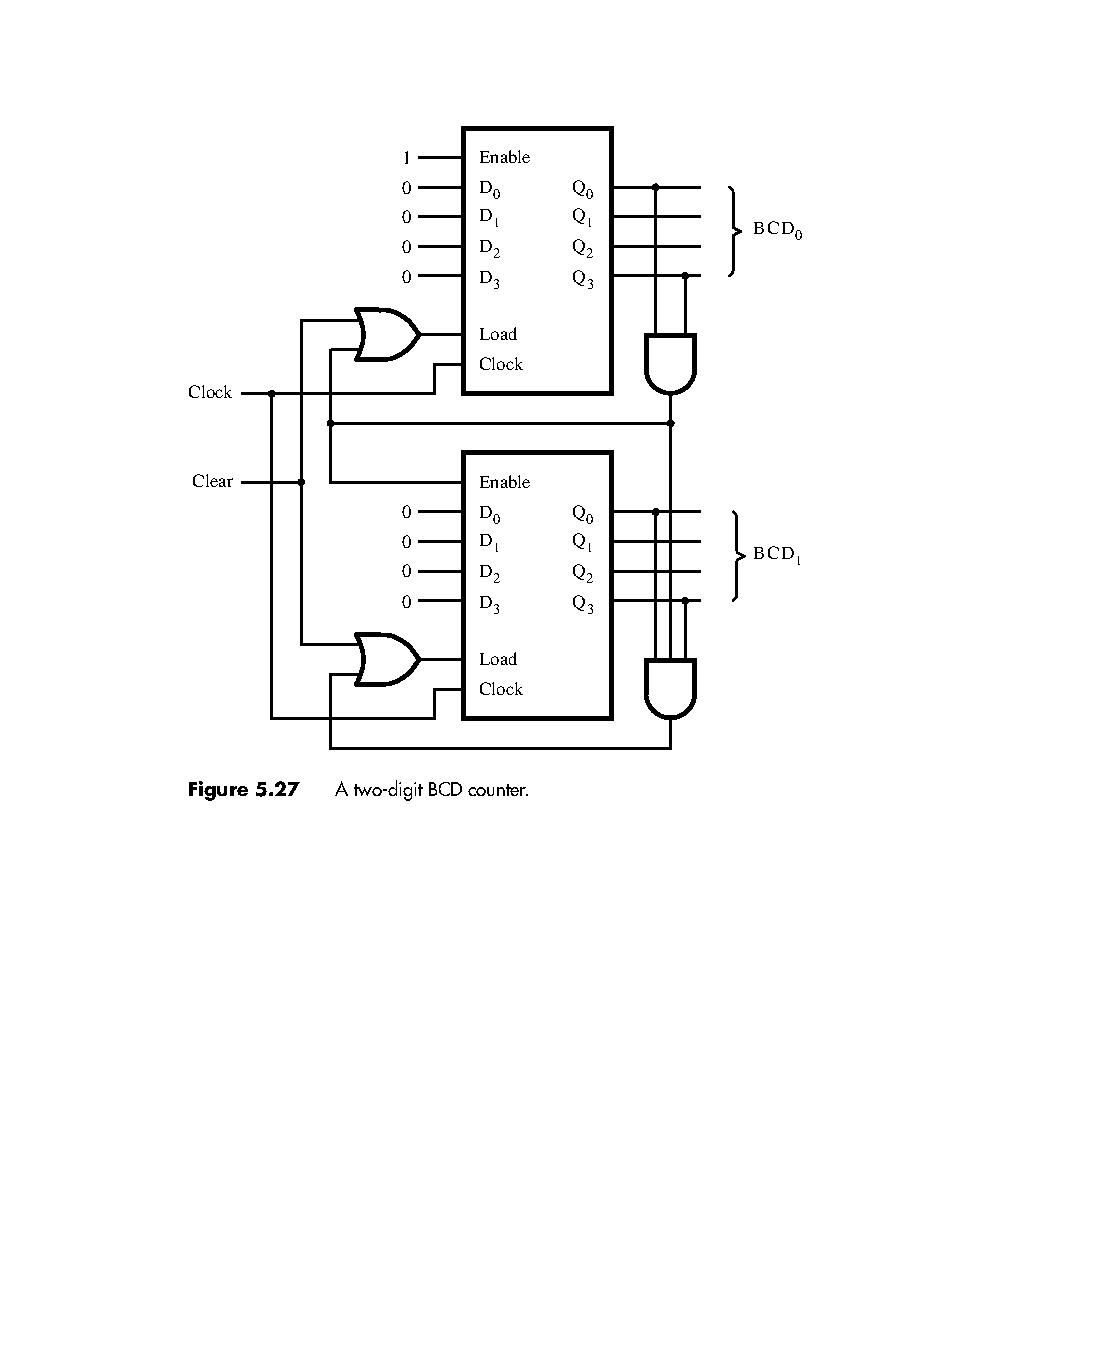
\includegraphics[height=.95\textheight]{VerilogFig5_27} \\
\end{frame}

\begin{frame}{Contador em anel}   \centering
    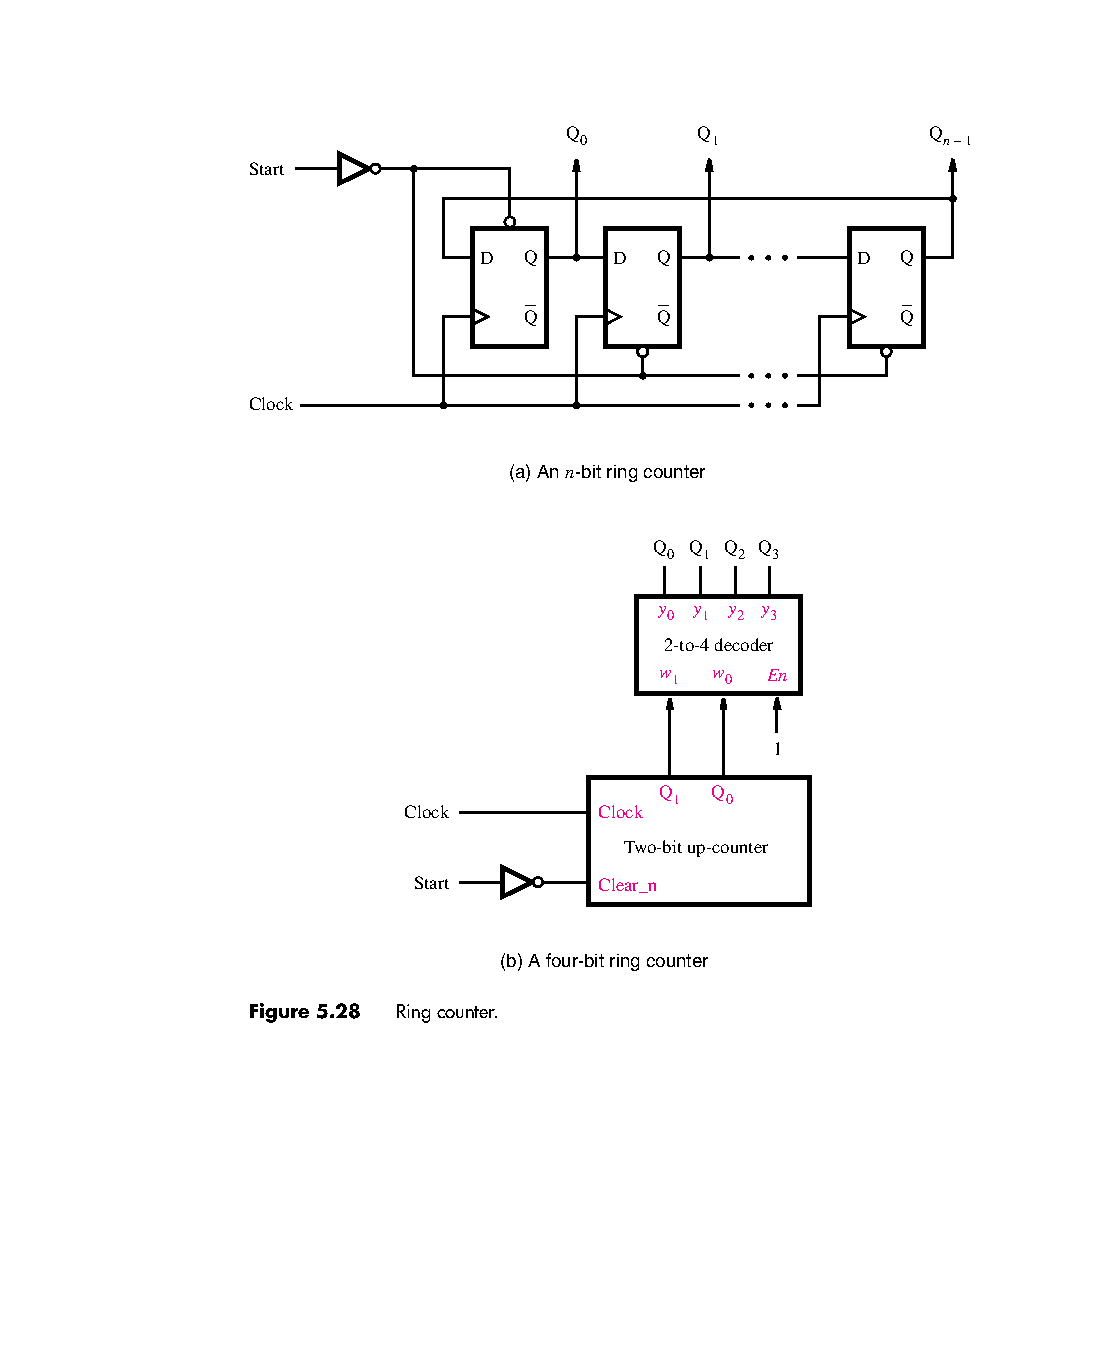
\includegraphics[height=.95\textheight]{VerilogFig5_28} \\
\end{frame}

\begin{frame}{Contador Johnson}   \centering
    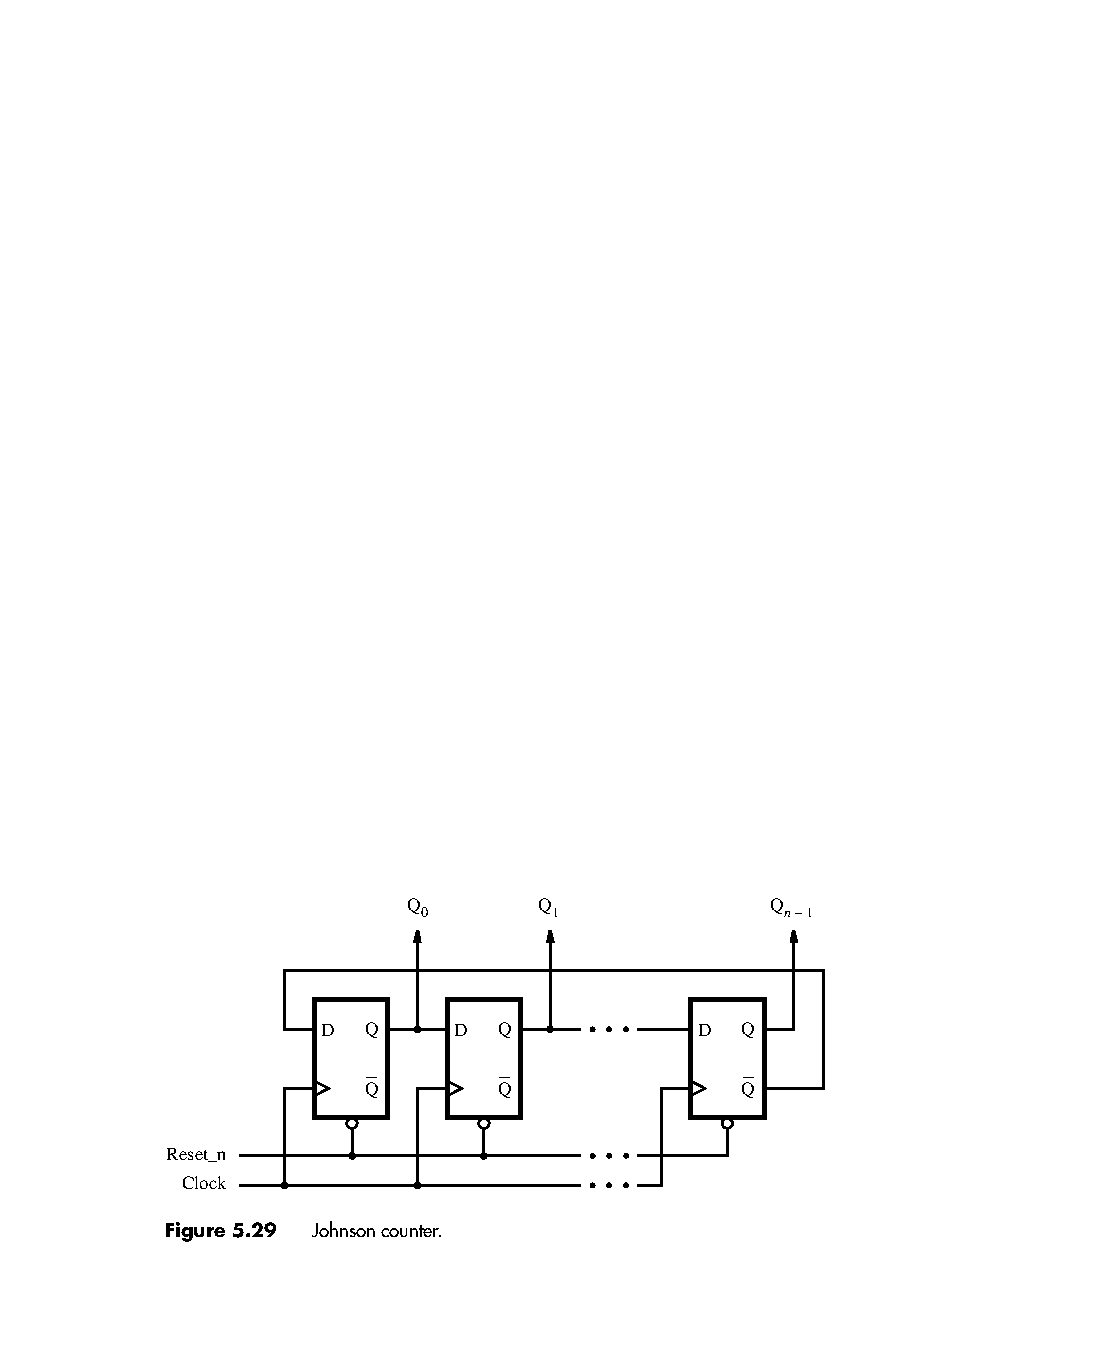
\includegraphics[height=.95\textheight]{VerilogFig5_29} \\
\end{frame}



\begin{frame}{Bibliografia} 
	\begin{itemize}
		\item \href{https://www.google.com.br/search?q=filetype\%3Apdf+Fundamentals+of+Digital+Logic+with+Verilog+Design+&oq=filetype\%3Apdf}{Brown, S. \& Vranesic, Z. - Fundamentals of Digital Logic with Verilog Design, 3rd Ed., Mc Graw Hill, 2009}
		\item \href{https://tams-www.informatik.uni-hamburg.de/applets/hades/}{https://tams-www.informatik.uni-hamburg.de/applets/hades/}
	\end{itemize}
\end{frame}

\begin{frame}
	\titlepage
\end{frame} 


\end{document}